
\section{Gedämpfte Schwingungen}

\subsection{Dämpfung mit konstanter Reibungskraft}

\vspace{-0.2cm}

$$ m \ddot{x}(t) = -k x(t) - \mu F_N \quad \text{für } \dot{x}(t) > 0 $$
$$ m \ddot{x}(t) = -k x(t) + \mu F_N \quad \text{für } \dot{x}(t) < 0 $$

\smallskip

\begin{minipage}[c]{0.7\columnwidth}
    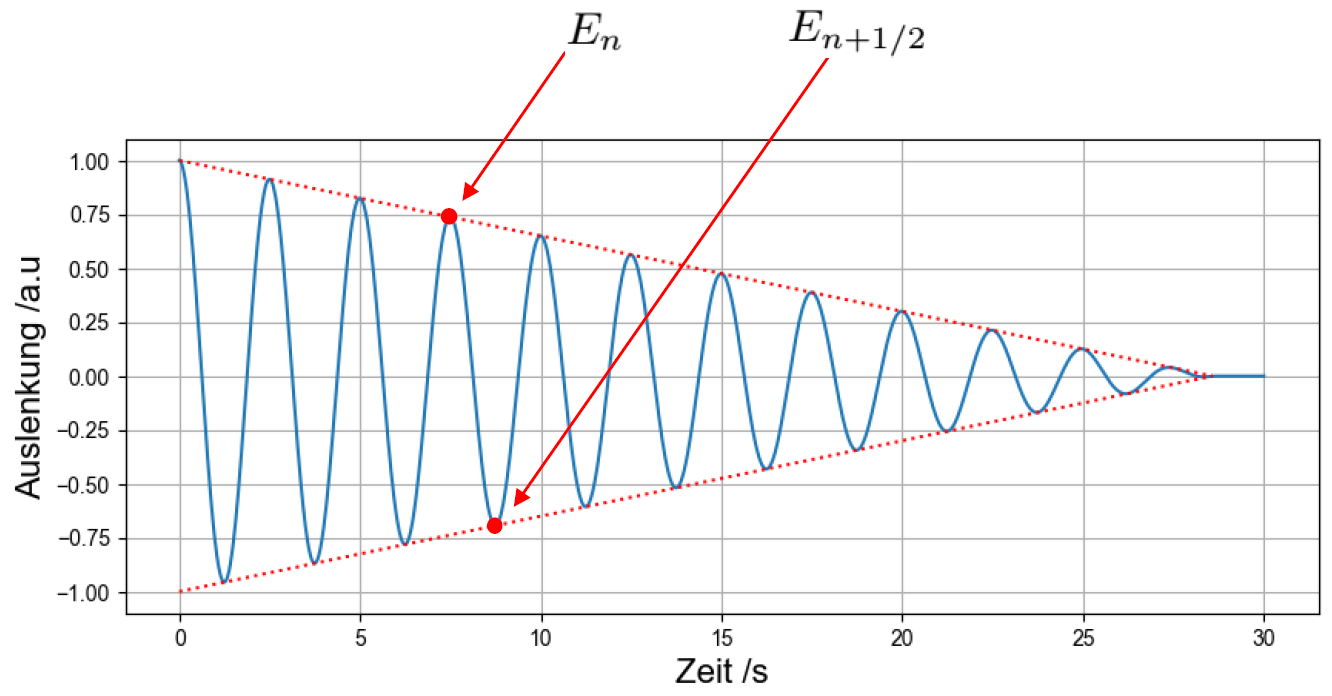
\includegraphics[width=\columnwidth]{images/gedaempfte_schwingungen_konst_reibung.png}
\end{minipage}
\hfill
\begin{minipage}[c]{0.28\columnwidth}
    $$ \boxed{ E = \frac{k \, A^2}{2} } $$
    $$ \boxed{ \Delta A = 4 \frac{F_R}{k}} $$
\end{minipage}


\begin{ctabular}{c l c}
    $E$         & Energie bei max. Auslenkung       & $[E] = \joule$                    \\
    $k=c$       & Federkonstante                    & $[k] = \frac{\newton}{\meter}$    \\
    $A$         & Amplitude bei max. Auslenkung     & $[A] = \meter$                    \\
    $\Delta A$  & Amplitudenänderung pro Periode    & $[\Delta A] = \meter$             \\
    $F_R$       & Reibungskraft                     & $[F_R] = \newton$ 
\end{ctabular}


\subsection{Dämpfung proportional zur Geschwindigkeit}

\vspace{-0.2cm}
\[
    m \ddot{x}(t) = -c \, x(t) - b \, \dot{x}(t)
    \quad \Rightarrow \quad
    \boxed{ \ddot{x}(t) + 2 \delta \, \dot{x}(t) + \omega_0^2 \, x(t) = 0 }
\]
\[
    \boxed{ \delta = \frac{b}{2m} = \frac{\kappa}{2} }
    \qquad
    \boxed{ \omega_0 = \sqrt{\frac{c}{m}} }
    \qquad
    \boxed{ D = \frac{\delta}{\omega_0} }
\]
\[
    \text{Charakt. Polynom:} \quad
    \lambda^2 + 2 \delta \lambda + \omega_0^2 = 0
    \quad \Rightarrow \quad
    \boxed{ \lambda_{1,2} = -\delta \pm \sqrt{\delta^2 - \omega_0^2} }
\]

\resizebox{\columnwidth}{!}{
    \begin{tabular}{llll}
        \toprule
        \textbf{Fall}                                   & $\bm{\lambda}$                                    & $\bm{x(t)}$                                                       & \textbf{Verhalten}                    \\
        \midrule
        $D < 1$ \; unterkritisch                        & $-\delta \pm i\,\Omega$ \; (2 komplexe)           & $A e^{-\delta t} \cos \left( \Omega t + \varphi \right)$          & gedämpfte Schwingung                  \\
        $D = 1$ \; kritisch                             & $-\delta$ \; (1 reelle)                           & $(A + B t) \, e^{-\delta t}$                                      & aperiodischer Grenzfall               \\
        $D > 1$ \; überkritisch                         & $-\delta \pm \sqrt{\delta^2 - \omega_0^2}$ \; (2 reelle) & $A e^{\lambda_1 t} + B e^{\lambda_2 t}$                    & aperiodisch (Kriechfall)              \\
        \bottomrule
    \end{tabular}
}

\smallskip
\centerline{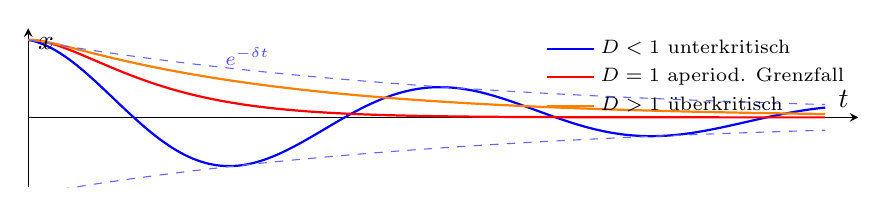
\begin{tikzpicture}
  \begin{axis}[
      width=\columnwidth, height=3.6cm,
      axis lines=middle, xmin=0, xmax=12.5, ymin=-0.9, ymax=1.15,
      xlabel={$t$}, ylabel={$x$}, ticks=none,
      samples=200, domain=0:12,
      legend style={font=\scriptsize, draw=none, fill=none, at={(1,1)}, anchor=north east},
      legend cell align=left,
    ]
    % omega_0 = 1, x(0) = 1, v(0) = 0
    \addplot[thick, blue]   {exp(-0.15*x)*cos(deg(0.989*x))};
    \addlegendentry{$D<1$ unterkritisch}
    \addplot[thick, red]    {(1+x)*exp(-x)};
    \addlegendentry{$D=1$ aperiod. Grenzfall}
    \addplot[thick, orange] {1.077*exp(-0.268*x) - 0.077*exp(-3.732*x)};
    \addlegendentry{$D>1$ überkritisch}
    \addplot[dashed, blue!60, forget plot] {exp(-0.15*x)};
    \addplot[dashed, blue!60, forget plot] {-exp(-0.15*x)};
    \node[blue!70, font=\scriptsize] at (axis cs:3.3,0.78) {$e^{-\delta t}$};
  \end{axis}
\end{tikzpicture}
}

$A$, $B$, $\varphi$ aus den Anfangsbedingungen $x(0)$, $\dot{x}(0)$. Der Grenzfall $D = 1$ kehrt am schnellsten ohne Überschwingen in die Ruhelage zurück.

\subsubsection{Unterkritischer Fall ($D < 1$)}

\vspace{-0.2cm}
\[
    \boxed{ \Omega = \sqrt{\omega_0^2 - \delta^2} = \omega_0 \sqrt{1 - D^2} }
    \qquad
    \boxed{ T = \frac{2 \pi}{\Omega} }
    \qquad
    \boxed{ f = \frac{\Omega}{2 \pi} }
\]
\[
    \text{Log. Dekrement:} \quad
    \boxed{ \Lambda = \ln \frac{A_n}{A_{n+1}} = \delta \, T }
    \qquad
    \ln \frac{A_n}{A_{n+\cbl{z}}} = \cbl{z} \, \Lambda
\]
\[
    \text{Aus } \Lambda \text{ und } \omega_0: \quad
    \boxed{ T = \frac{\sqrt{4\pi^2 + \Lambda^2}}{\omega_0} }
\]

\begin{ctabular}{c l c}
    $b$         & Dämpfungskonstante ($F_R = -b\,\dot{x}$)  & $[b] = \frac{\newton \, \second}{\meter}$ \\
    $c = k$     & Federkonstante                            & $[c] = \frac{\newton}{\meter}$            \\
    $\delta$    & Abklingkonstante                          & $[\delta] = \frac{1}{\second}$            \\
    $\kappa$    & $\kappa = b/m = 2\delta$                  & $[\kappa] = \frac{1}{\second}$            \\
    $\omega_0$  & Kreisfrequenz ungedämpfte Schwingung      & $[\omega_0] = \frac{\rad}{\second}$       \\
    $D$         & Dämpfungsgrad                             & $[D] = 1$                                 \\
    $\Omega$    & Kreisfrequenz gedämpfte Schwingung        & $[\Omega] = \frac{\rad}{\second}$         \\
    $T$         & Periodendauer gedämpfte Schwingung        & $[T] = \second$                           \\
    $\Lambda$   & Logarithmisches Dekrement                 & $[\Lambda] = 1$                           \\
    $A_n$       & $n$-te Maximalamplitude                   & $[A_n] = \meter$                          \\
    $\cbl{z}$         & Anzahl verstrichene Perioden              & $[z] = 1$
\end{ctabular}
